\documentclass[11pt]{article}

\usepackage{fullpage}

\usepackage{amsmath, amsfonts}

\usepackage{etoolbox}

\usepackage{graphicx}

\providetoggle{solution}

%\togglefalse{solution}

\toggletrue{solution}

\title{CS4780/5780 Homework 1 Solution}

\author{}

\date{}

\begin{document}

    \maketitle

    \section*{Problem 1: Train/Test Splits}

    \begin{enumerate}

        \item We split the training data by person - for example, we can allocate 80\% of the images as the training set, then 10\% each for the validation and test sets respectively. It is critical that there is no overlap among three datasets, as the different datasets should be independent from one another.

        \item If you solely used the additional dataset on the well-trained model, then it would go wrong that there will be bias towards these 5 categories among your results. As the system will be used to identify more objects, we can use all of the original training dataset along with, for example, 80\% of additional images to form the new training set - ideally we want roughly equal numbers of images per category. Then, the remaining 20\% of the additional images can be split equally and merged into the original test and validation sets. (Other percentage splits are acceptable if reasonable.)

    \end{enumerate}
    \section*{Problem 2: K-nearest Neighbors}

	\begin{enumerate}
		\item See figure 1. Blue = positive, Yellow = negative, Red = boundary line.
		\begin{figure}[h!]
			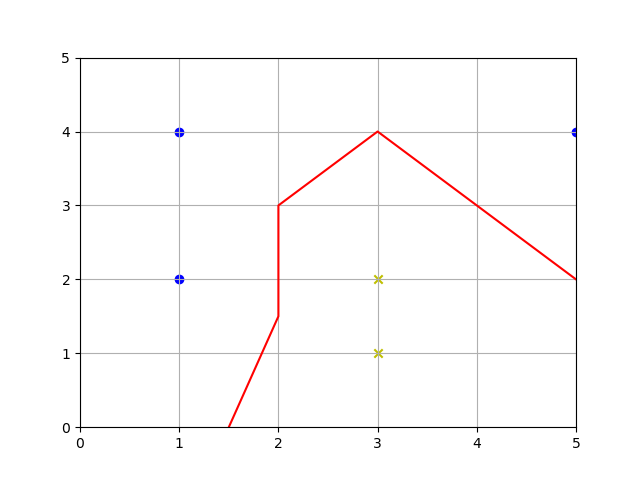
\includegraphics[width=8cm]{Graph1_solution.png}
			\centering
			\caption{Decision boundary for 1-NN }
		\end{figure}
		
		\item She will classify (500, 1) as $+1$ with the given 1-NN classifier since the point is closest to the point (500, 4).\\ For original test point $(5, 1)$, she will predict $-1$ because the point is closest to $(3, 1)$
		\item Since we are performing 2-NN, the two closest points by Euclidean distance are (0, 0) and (1, 1), each with labels 1.0, 2.5 respectively. Since this is a regression problem, we take the average of these two labels and return 1.75 as our answer.
		\item Yes, we can remove those features vectors that have missing values and use K-NN on the new dataset.
		\item Unless there is serious preprocessing done on the training data that aids in distance computation,
		applying a k-NN classifier will take more time: training consists solely of storing the points, while
		applying must compute the distance between the test point and all stored training points.
		
		\item K-NN still works on images because the underlying latent representation behind images is of low dimension - the curse of dimensionality only takes hold on data with high latent dimensionality.
		
	\end{enumerate}

\section*{Problem 3: Curse of Dimensionality}
	For general $d$, $\frac{V_d(r_1)}{V_d(r_2)} = \frac{\frac{\pi^{\frac{d}{2}}}{\Gamma(\frac{d}{2} + 1)}r_1^d} {\frac{\pi^{\frac{d}{2}}}{\Gamma(\frac{d}{2} + 1)}r_2^d} = \left(\frac{r_1}{r_2}\right)^{d}$.
	\begin{enumerate}
		\item $\frac{V_3(0.99r)}{V_3(r)} = \left(0.99\right)^3 \approx 0.97$
		\item $\frac{V_{10000}(0.99r)}{V_{10000}(r)} = \left(0.99\right)^{10000} \approx 2.24*10^{-44} \approx 0$
	\end{enumerate}
	Although the ratio is decreased by only $1\%$, the relative volume of remaining ball is very tiny when the dimension is high.
\end{document}

